\documentclass[a4paper,10pt]{article}

\usepackage[T1]{fontenc}
\usepackage[utf8]{inputenc}
\usepackage{graphicx}
\usepackage{xcolor}
\usepackage{fourier}
\usepackage{caption}
\usepackage{subcaption}

\usepackage{tgtermes}

\usepackage[
pdftitle={Statistical Machine Learning}, 
pdfauthor={Inez Wijnands \& Guido Zuidhof, Radboud University Nijmegen},
colorlinks=true,linkcolor=blue,urlcolor=blue,citecolor=blue,bookmarks=true,
bookmarksopenlevel=2]{hyperref}
\usepackage{amsmath,amssymb,amsthm,textcomp}
\usepackage{enumerate}
\usepackage{multicol}
\usepackage{tikz}

\usepackage{geometry}
\geometry{total={210mm,297mm},
left=25mm,right=25mm,%
bindingoffset=0mm, top=20mm,bottom=20mm}

\numberwithin{equation}{section} % Number equations within sections (i.e. 1.1 instead of 1)
\numberwithin{figure}{section} % Number figures within sections (i.e. 1.1 i/o 1)
\numberwithin{table}{section} % Number tables within sections (i.e. 1.1 i/of 1)

\linespread{1.35}

\newcommand{\linia}{\rule{\linewidth}{0.5pt}}

% custom theorems if needed
\newtheoremstyle{mytheor}
    {1ex}{1ex}{\normalfont}{0pt}{\scshape}{.}{1ex}
    {{\thmname{#1 }}{\thmnumber{#2}}{\thmnote{ (#3)}}}

\theoremstyle{mytheor}
\newtheorem{defi}{Definition}

% my own titles
\makeatletter
\renewcommand{\maketitle}{
\begin{center}
\vspace{2ex}
{\huge \textsc{\@title}}
\vspace{1ex}
\\
\linia\\
\@author  \@date
\vspace{4ex}
\end{center}
}
\makeatother
%%%

% custom footers and headers
\usepackage{fancyhdr,lastpage}
\pagestyle{fancy}
\lhead{}
\chead{}
\rhead{}
\lfoot{Assignment \textnumero{} 2}
\cfoot{}
\rfoot{Page \thepage\ /\ \pageref*{LastPage}}
\renewcommand{\headrulewidth}{0pt}
\renewcommand{\footrulewidth}{0pt}
%

% code listing settings
\usepackage{listings}
\lstset{
    language=Python,
    basicstyle=\ttfamily\small,
    aboveskip={0.9\baselineskip},
    belowskip={0.9\baselineskip},
    columns=fixed,
    extendedchars=true,
    breaklines=true,
    tabsize=4,
    prebreak=\raisebox{0ex}[0ex][0ex]{\ensuremath{\hookleftarrow}},
    frame=lines,
    showtabs=false,
    showspaces=false,
    showstringspaces=false,
    keywordstyle=\color[rgb]{0.1,0.126,0.941},
    commentstyle=\color[rgb]{0.133,0.545,0.133},
    stringstyle=\color[rgb]{0,0.5,0},
    numbers=left,
    numberstyle=\scriptsize\ttfamily,
    stepnumber=1,
    numbersep=10pt,
    captionpos=t,
    escapeinside={\%*}{*)}
}

%%%----------%%%----------%%%----------%%%----------%%%

\begin{document}

\title{Statistical Machine Learning \\ Assignment 2}

\author{Inez Wijnands (s4149696) \& Guido Zuidhof (s4160703)\\ Radboud University Nijmegen\\}

\date{04/11/2015}

\maketitle

\noindent \textit{The entire code listing is in a separate file. The listings shown here are merely code snippets}.\vspace{-0.5cm}
\section{Sequential learning}
\subsection{Obtaining the prior}
\begin{enumerate}
	\item \begin{align}
			\boldsymbol{\tilde \Lambda}_{a,b} &= \boldsymbol{\tilde \Sigma}_{a,b}^{-1} \\
			&= \newcommand*{\temp}{\multicolumn{1}{c|}{}} 
				 \begin{pmatrix}
					60&50&\temp&-48&38\\ 
					50&50&\temp&-50&40\\ \cline{1-5} 
					-48&-50&\temp&52.4&-41.4 \\
					38&40&\temp&-41.4&33.4
				\end{pmatrix}
		\end{align}\\\\
		Using the precision matrix $\boldsymbol{\tilde \Lambda}$ we can use equations 2.69, 2.73 and 2.75 from Bishop to obtain the mean and covariance of the conditional distribution $p([x_1,x_2]^T|x_3 = x_4 = 0)$.\\
		\begin{align}
			\boldsymbol{\Sigma}_p &= \boldsymbol \Lambda_{aa}^{-1} \tag{Bishop 2.73}\\
			\boldsymbol \Lambda_{aa} &= \begin{pmatrix} 60 & 50 \\ 50 & 50 \end{pmatrix}\\
			\boldsymbol{\Sigma}_p &= \begin{pmatrix} 0.1 & -0.1 \\ -0.1 & 0.12 \end{pmatrix}
		\end{align}
		\begin{align}
			\boldsymbol{\mu}_p = \boldsymbol{\mu}_{a | b} = \boldsymbol{\mu}_a - \boldsymbol{\Lambda}_{aa}^{-1}\boldsymbol{\Lambda}_{ab}(\boldsymbol{x}_b - \boldsymbol{\mu}_b) \tag{Bishop 2.75}
		\end{align}
		We can fill in this equation, since $\boldsymbol {\tilde \mu}$ and $\boldsymbol x_b$ (the second partition of $\boldsymbol x$) are known.
		\begin{align}
			\boldsymbol{\mu}_p &=
			\begin{pmatrix} 1\\ 0 \end{pmatrix}-
			\begin{pmatrix} 60 & 50 \\ 50 & 50 \end{pmatrix}^{-1}
			\begin{pmatrix} -48 & 38\\ -50 & 40 \end{pmatrix}
			(\begin{pmatrix} 0\\ 0 \end{pmatrix}-
			\begin{pmatrix} 1\\ 2 \end{pmatrix}) \\
			&= \begin{pmatrix} 1\\ 0 \end{pmatrix}-
			\begin{pmatrix} 0.1 & -0.1 \\ -0.1 & 0.12 \end{pmatrix}
			\begin{pmatrix} -48 & 38\\ -50 & 40 \end{pmatrix}
			(\begin{pmatrix} 0\\ 0 \end{pmatrix}-
			\begin{pmatrix} 1\\ 2 \end{pmatrix}) \\
			&= \begin{pmatrix} 0.8\\ 0.8 \end{pmatrix}
		\end{align}
	\item Using the prior $\boldsymbol \mu_p$ and $\boldsymbol \Sigma_p$, we used the numpy-equivalent in Python for the MATLAB-function \verb|mvnrnd| to obtain the $\boldsymbol \mu_t$ we used for the remainder of this assignment:
		\begin{verbatim}
			np.random.multivariate_normal(mu_p, sigma_p, 1)
		\end{verbatim}
		This resulted in:
		\begin{equation}
			\boldsymbol\mu_t = \begin{pmatrix} 0.28584241 \\ 1.42626702\end{pmatrix}
		\end{equation}
	\item The probability density is highest at the mean (as illustrated in Figure 1.1). The density decreases quickly as both x and y change, but less so when $x$ XOR $y$ change. In $\boldsymbol \Sigma_p$, the values for the $x$ XOR $y$ are lower, so this is consistent with our density plot.
		\begin{figure}[h!]
   			\centering
   			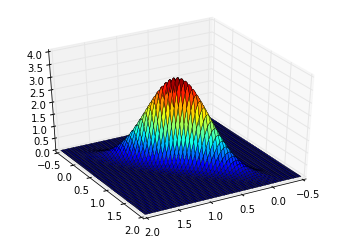
\includegraphics{probdens.png}\vspace{-0.2cm}
   			\caption{\vspace{-0.2cm} The probability density of the distribution.}
  		\end{figure}
\end{enumerate}

\subsection{Generating the data}
\begin{enumerate}
	\item We used the following function to generate our data:
	\begin{verbatim}
		np.random.multivariate_normal(mu_t, sigma_t, 1000)
	\end{verbatim}
	\item \begin{align}\boldsymbol{\mu}_{ML} &= \frac{1}{N}  \sum_{n=1}^{N} \boldsymbol{x}_n \tag{Bishop 2.121}\\ 
	&= [\frac{1}{1000}  \sum_{n=1}^{1000} \boldsymbol{x}_n, \frac{1}{1000}  \sum_{n=1}^{1000} \boldsymbol{y}_n]\\
	&= \begin{pmatrix}
0.25383138\\
1.38260838
\end{pmatrix}
		\end{align}
		\begin{align}
		\boldsymbol{\Sigma}_{ML} &= \frac{1}{N} \sum_{n=1}^{N} (\boldsymbol{x}_n - \boldsymbol{\mu}_{ML})(\boldsymbol{x}_n - \boldsymbol{\mu}_{ML})^T \tag{Bishop 1.22}\\
		&= \begin{pmatrix}
\frac{1}{1000} \sum_{n=1}^{1000} (\boldsymbol{x}_n - \boldsymbol{\mu}_{(1)ML})(\boldsymbol{x}_n - \boldsymbol{\mu}_{(1)ML})^T & \frac{1}{1000} \sum_{n=1}^{1000} (\boldsymbol{x}_n - \boldsymbol{\mu}_{(1)ML})(\boldsymbol{y}_n - \boldsymbol{\mu}_{(2)ML})^T\\
\frac{1}{1000} \sum_{n=1}^{1000} (\boldsymbol{y}_n - \boldsymbol{\mu}_{(2)ML})(\boldsymbol{x}_n - \boldsymbol{\mu}_{(1)ML})^T & \frac{1}{1000} \sum_{n=1}^{1000} (\boldsymbol{y}_n - \boldsymbol{\mu}_{(2)ML})(\boldsymbol{y}_n - \boldsymbol{\mu}_{(2)ML})^T
\end{pmatrix}\\
		&= \begin{pmatrix}
1.90513804 & 0.72479489\\
0.72479489 & 3.81690496
\end{pmatrix}
		\end{align}
		This is calculated using the code in Listing 1:
		\begin{lstlisting}[label={list:first},caption=Python code to calculate $\boldsymbol \mu_{ML}$ and $\boldsymbol \Sigma_{ML}$.]
mu_ml = sum(data)/len(data)

sse = [0,0]
for point in data:
        	point = np.matrix(point)
        	sse += (point-mu_ml).T*(point-mu_ml)
sigma_ml =  sse/len(data)
    		\end{lstlisting}
    		The differences with the 'true' values are:
    		\begin{align}
    		\boldsymbol \mu_t - \boldsymbol \mu_{ML} &= \begin{pmatrix} 0.28584241 \\ 1.42626702\end{pmatrix} - \begin{pmatrix} 0.25383138\\ 1.38260838 \end{pmatrix} = \begin{pmatrix} 0.03201103\\ 0.04365864 \end{pmatrix}\\
    		\boldsymbol \Sigma_t - \boldsymbol \Sigma_{ML} &= \begin{pmatrix} 2.0 & 0.8\\ 0.8 & 4.0 \end{pmatrix} - \begin{pmatrix} 1.90513804 & 0.72479489\\ 0.72479489 & 3.81690496 \end{pmatrix} = \begin{pmatrix} 0.09486196 & 0.07520511\\ 0.07520511 & 0.18309504 \end{pmatrix}
		\end{align}
\end{enumerate}
		For the unbiased covariance:
		\begin{equation}
		\boldsymbol {\tilde \Sigma} = \frac{1}{N-1} \sum_{n=1}^N (\boldsymbol x_n - \boldsymbol \mu_{ML})(\boldsymbol x_n - \boldsymbol \mu_{ML})^T \tag{Bishop 2.125}
		\end{equation}
		We added this line of code to the function of Listing 1:
		\begin{verbatim}
			sigma_ml_unbiased = sse * (1/(len(data)-1))
		\end{verbatim}
		The difference between the unbiased covariance and the 'true' covariance is:
		\begin{equation} 
		\boldsymbol \Sigma_t - \boldsymbol{\tilde \Sigma} = \begin{pmatrix} 2.0 & 0.8\\ 0.8 & 4.0 \end{pmatrix} - \begin{pmatrix} 1.90704509 & 0.72552041\\ 0.72552041 & 3.82072569 \end{pmatrix} = \begin{pmatrix} 0.09295491 & 0.07447959\\ 0.07447959 & 0.17927431 \end{pmatrix}
		\end{equation}
		The difference is slightly smaller than the difference between $\boldsymbol \Sigma_t$ and $\boldsymbol \Sigma_{ML}$. 

\subsection{Sequential learning algorithms}
\begin{enumerate}
	\item See Listing 2 for our procedure to process all data points one-by-one to calculate an estimate of $\boldsymbol \mu_{ML}$. \begin{lstlisting}[label={list:first},caption=Python code for function \textit{sequential\_learning\_ml(data)}.]
def sequential_learning_ml(data):
    N = 0
    mu_ml = 0
    mus = []

    for point in data:
        N += 1
        mu_ml = mu_ml + (1/N)*(point-mu_ml)
        mus.append(mu_ml)

    print "Sequential mu_ml:", mu_ml
    return mus
    		\end{lstlisting}
    		This resulted in:
    		\begin{equation}
    		\boldsymbol \mu_{ML} = \begin{pmatrix} 0.25383138 \\ 1.38260838 \end{pmatrix}
    		\end{equation}
	\item \begin{equation}p(\boldsymbol{x} | D_{n-1}) = \mathcal{N}(\boldsymbol{x} | \boldsymbol{\mu}, \boldsymbol{\Lambda}^{-1}) \tag{Bishop 2.113}
		\end{equation}
where: $\boldsymbol{x} = \boldsymbol{\mu}, \boldsymbol{\mu} = \boldsymbol{\mu}_{(n-1)}, \boldsymbol{\Lambda}^{-1} = \boldsymbol{\Sigma}_{(n-1)}$
		\begin{equation}p(\boldsymbol{y} | \boldsymbol{x}) = \mathcal{N}(\boldsymbol{y} | \boldsymbol{Ax} + \boldsymbol{b}, \boldsymbol{L}^{-1}) \tag{Bishop 2.114}
		\end{equation}
where $\boldsymbol{y} = \boldsymbol{x}_n, \boldsymbol{A} = \boldsymbol{I}, \boldsymbol{x} = \boldsymbol{\mu}, \boldsymbol{b} = 0, \boldsymbol{L}^{-1} = \boldsymbol{\Sigma}^t$
		\begin{align} p(\boldsymbol{x} | \boldsymbol y) &= \mathcal{N}(\boldsymbol{x} | \boldsymbol{\Sigma} \{ \boldsymbol{A}^T \boldsymbol{L}(\boldsymbol{y} - \boldsymbol{b}) + \boldsymbol{\Lambda\mu}\}, \boldsymbol{\Sigma}) \tag{Bishop 2.116}\\
	 	\boldsymbol{\Sigma} &= (\boldsymbol{\Lambda} + \boldsymbol{A}^T\boldsymbol{LA})^{-1} \tag{Bishop 2.117}
	 	\end{align}
		Matching the variables we get the following equations:
		\begin{align}
			p(\boldsymbol{\mu} | \boldsymbol{x}_n) &= \mathcal{N}(\boldsymbol{\mu} | \boldsymbol S \{ \boldsymbol{I}^T \boldsymbol{\Sigma}_t^{-1}(\boldsymbol{x}_n - 0) + \boldsymbol{\Sigma}_{(n-1)}^{-1}\}, \boldsymbol S)\\
			&= \mathcal{N}(\boldsymbol{\mu} | \boldsymbol S \{ \boldsymbol{I}^T \boldsymbol{\Sigma}_t^{-1} \boldsymbol{x}_n + \boldsymbol{\Sigma}_{(n-1)}^{-1}\}, \boldsymbol S)\\
			 &= \mathcal{N}(\boldsymbol{\mu} | \boldsymbol S \{ \boldsymbol{\Sigma}_t^{-1} \boldsymbol{x}_n + \boldsymbol{\Sigma}_{(n-1)}^{-1}\}, \boldsymbol S)\\
			\boldsymbol{S} &= (\boldsymbol{\Sigma}_{(n-1)}^{-1} + \boldsymbol{I}^T \boldsymbol{\Sigma}_t^{-1} \boldsymbol{I})^{-1}\\
			&= (\boldsymbol{\Sigma}_{(n-1)}^{-1} + \boldsymbol{\Sigma}_t^{-1})^{-1}
		\end{align}
		$\boldsymbol \mu_n$ is the mean of the distribution $p(\boldsymbol \mu | \boldsymbol x_n)$, so the functions we use for our sequential learning algorithm are:
		\begin{align}
			\boldsymbol \Sigma_n &= \boldsymbol S\\
			\boldsymbol \mu_n &= \boldsymbol \Sigma_n \{ \boldsymbol \Sigma_t^{-1} \boldsymbol x_n + \boldsymbol{\Sigma}_{n-1}^{-1}\}, \boldsymbol \Sigma_n)
		\end{align}
	\item See Listing 3 for our procedure to make a MAP estimation of $\boldsymbol \mu$ by processing the data points one-by-one. \\
	\begin{lstlisting}[label={list:first},caption=Python code for function \textit{sequential\_learning\_map(data, mu\_p, sigma\_p, sigma\_t)}.]
def sequential_learning_map(data, mu_p, sigma_p, sigma_t):
    sigma = sigma_p
    mu = mu_p
    mus = []

    for point in data:
        point = np.matrix(point).T
        S =  np.linalg.inv( np.linalg.inv(sigma) + np.linalg.inv(sigma_t))
        mu = np.dot(S, np.dot( np.linalg.inv(sigma_t), point) + np.dot( np.linalg.inv(sigma),  mu))
        sigma = S
        mus.append(np.array(mu))

    print "Sequential mu_map:", mu
    return mus
    		\end{lstlisting}
    		This resulted in:
    		\begin{equation}
    		\boldsymbol \mu_{MAP} = \begin{pmatrix} 0.25941079 \\ 1.37796331 \end{pmatrix}
    		\end{equation}
	\item See Figure 1.2 for our results: \begin{figure}[h!]
   			\centering
   			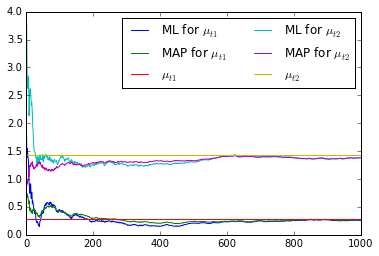
\includegraphics{mu.png}\vspace{-0.2cm}
   			\caption{\vspace{-0.2cm} The ML and MAP estimates for $\boldsymbol \mu$ are given, plotted against the amount of data points observed. The 'true' value $\boldsymbol \mu_t$ is also indicated. This is done for both $\boldsymbol \mu_{t1}$ and $\boldsymbol \mu_{t2}$. }
  		\end{figure}
  		We observed that the MAP estimate performs better for less data points. This seems logical enough, since the MAP estimate is a regularized version of the ML estimate. When more data points are observed, the difference is almost non-existent.
\end{enumerate}

\vfill

\section{The faulty lighthouse}
\subsection{Constructing the model}
\begin{enumerate}
	\item A full circle is 360 degrees and correspond to 2$\pi$. Since the light house can only be observed from the coast, which is a straight line, the light can only reach half a circle. This means that we need to see if the distribution for the values $-\frac{1}{2}\pi$ to $\frac{1}{2}\pi$ adds up to one. If it is a reasonable distribution, the following should hold:
		\begin{align}
		\int_{-\frac{1}{2}\pi}^{\frac{1}{2}\pi} \frac{1}{\pi} dx &= 1\\
		&= \frac{x}{\pi} + c \bigg \vert_{-\frac{1}{2}\pi}^{\frac{1}{2}\pi}\\
		& = \frac{\frac{1}{2}\pi}{\pi} - \frac{-\frac{1}{2}\pi}{\pi} = 1
		\end{align}
		We can conclude that since the light of the lighthouse can reach half a circle, $\frac{1}{\pi}$ is a fine distribution (this means a uniform distribution over the possible angles).
	\item First, using the given $\beta \tan (\theta_k) = x_k - \alpha$, we will calculate the derivation of $\theta$.
		\begin{align}
		\beta \tan (\theta_k) &= x_k - \alpha \tag{Assignment eq. 7}\\
		\tan (\theta_k) &= \frac{x_k - \alpha}{\beta} \\
		\theta_k &= \tan^{-1} \frac{x_k - \alpha}{\beta} \\
		\bigg \vert \frac{d\theta}{dx} \bigg \vert &= \frac{1}{1 + (\frac{x_k - \alpha}{\beta})^2} \cdot \bigg \vert \frac{d\frac{x_k - \alpha}{\beta}}{dx} \bigg \vert\\
		&= \frac{1}{1 + \frac{x_k - \alpha}{\beta}^2} \cdot \frac{\beta}{\beta^2}\\
		&= \frac{\beta}{\beta^2 + \beta^2(\frac{x_k - \alpha}{\beta})^2}\\
		&= \frac{\beta}{\beta^2 + \beta^2\frac{(x_k - \alpha)^2}{\beta^2}}\\
		& = \frac{\beta}{\beta^2 + (x_k - \alpha)^2}
		\end{align}
		Since the following equation holds:
		\begin{equation}
		p_x(x) = p_{\theta}(\theta_k)\bigg \vert \frac{d\theta}{dx} \bigg \vert \tag{Bishop 1.27}
		\end{equation}
		We need to multiply the derivation of $\theta$ with $p(\theta_k | \alpha, \beta)$ (Assignment eq. 6):
		\begin{align}
		p(x_k | \alpha, \beta) &= \frac{\beta}{\beta^2 + (x_k - \alpha)^2} \cdot \frac{1}{\pi}\\
		&= \frac{\beta}{\pi [\beta^2 + (x_k - \alpha)^2]} \tag{Assignment eq. 8}
		\end{align}
		We have plotted the distribution for $\beta$ = 1 and for $\alpha$ we chose the value 0.5, as illustrated in Figure 2.1: \begin{figure}[h!]
   			\centering
   			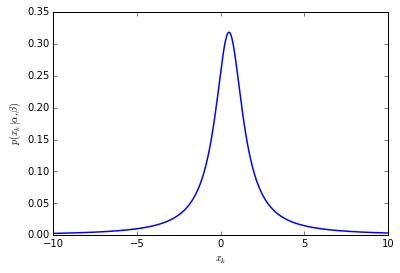
\includegraphics{distr.png}\vspace{-0.2cm}
   			\caption{\vspace{-0.2cm} The probability distribution $p(x_k | \alpha, \beta)$ plotted against $x_k$, with $\alpha = 0.5$ and $\beta = 1$.}
  		\end{figure}	
	\item \begin{align}
		p(\alpha | \mathcal{D}, \beta) &= p(\mathcal{D} | \alpha, \beta) p(\alpha | \beta)\\
		p(x_k | \alpha, \beta) &= \frac{\beta}{\pi[\beta^2 + (x_k - \alpha)^2]} \tag{Assignment eq. 8}\\
		&= \frac{\beta}{\pi} \cdot \frac{1}{\beta^2 + (x_k - \alpha)^2}\\
		\ln(p(x_k | \alpha, \beta)) &= \ln(\frac{\beta}{\pi} \cdot \frac{1}{\beta^2 + (x_k - \alpha)^2})\\
		&= \ln\frac{\beta}{\pi} + \ln(\frac{1}{\beta^2 + (x_k - \alpha)^2})\\
		&= \ln\frac{\beta}{\pi} - \ln[\beta^2 + (x_k - \alpha)^2]\\
		p(\mathcal{D} | \alpha, \beta) &= \prod_{x_k \in \mathcal{D}} p(x_k | \alpha, \beta)\\
		\ln(p(\mathcal{D} | \alpha, \beta)) &= \bigg \vert \mathcal{D}\bigg \vert \cdot \ln(\frac{\beta}{\pi}) - \sum_{x_k \in \mathcal{D}} \ln([x_k - \alpha)^2 + \beta^2])
		\end{align}
		Since $\bigg \vert \mathcal{D}\bigg \vert \cdot \ln(\frac{\beta}{\pi})$ is a constant, the log of the posterior density can be written like this:
		\begin{equation}
		\ln(p(\alpha | \mathcal{D}, \beta)) = \bigg \vert \mathcal{D}\bigg \vert \cdot \ln(\frac{\beta}{\pi}) - \sum_{x_k \in \mathcal{D}} \ln([x_k - \alpha)^2 + \beta^2]) \tag{Assignment eq. 9}
		\end{equation}
		Maximizing the posterior density gives the following expression:
		\begin{align}
		\hat \alpha &= \arg \max_\alpha [p(\mathcal{D} | \alpha, \beta)]\\
		&= \arg \max_\alpha [\prod_{x_k \in \mathcal{D}} p(x_k | \alpha, \beta)]\\
		&= \arg \max_\alpha [\prod_{x_k \in \mathcal{D}} \frac{\beta}{\pi[\beta^2 + (x_k - \alpha)^2]}]\\
		\end{align}
	\item \begin{figure}[h!]
   			\centering
   			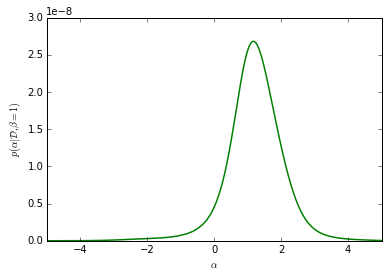
\includegraphics{alpharoni.png}\vspace{-0.2cm}
   			\caption{\vspace{-0.2cm} The probability density $p(\alpha | \mathcal{D}, \beta = 1)$ plotted against $\alpha$.}
  		\end{figure}
  		The most likely estimate for $\hat{\alpha}$ = 1.17136. The mean of $\alpha$ = -0.18333. The difference is probably caused by the amount of data points we have, these are very limited. Outliers in the data will have a great effect on the mean.
\end{enumerate}

\subsection{Generate the lighthouse data}
\begin{enumerate}
	\item 
	\item 
\end{enumerate}

\subsection{Find the lighthouse}
\begin{enumerate}
	\item
	\item 
	\item 
\end{enumerate}
\end{document}
